\section{Proposed Architecture}

\begin{figure}
    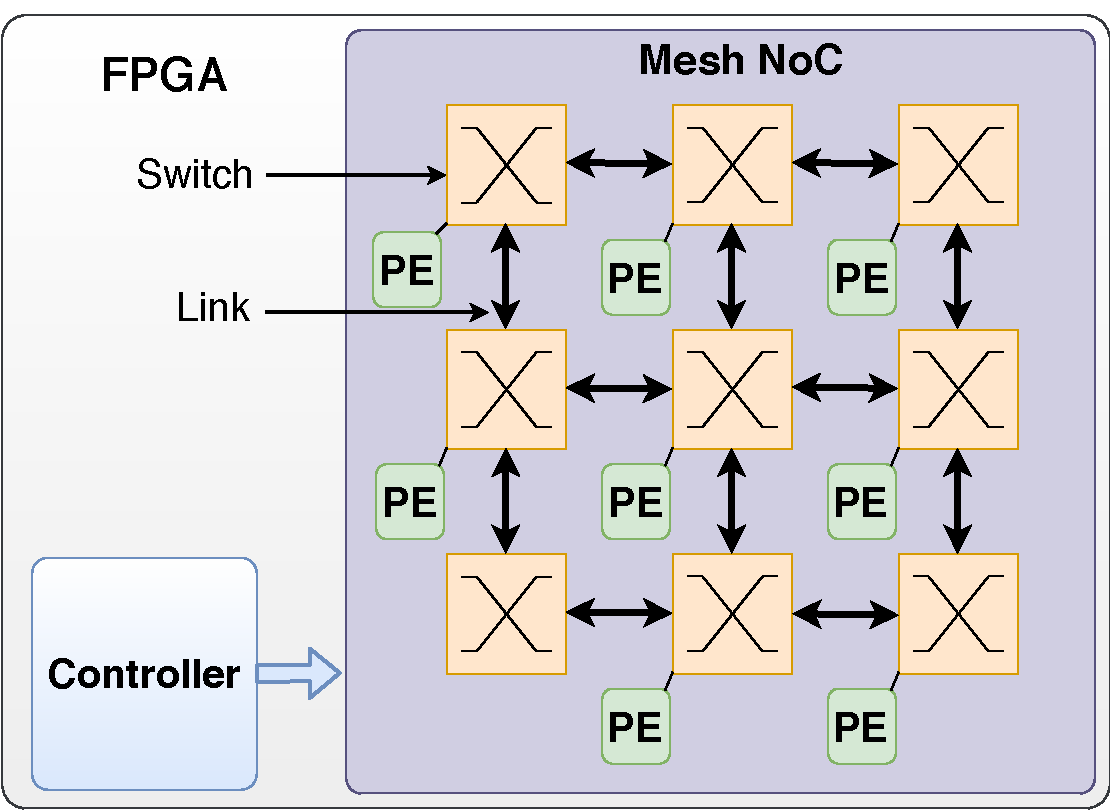
\includegraphics[width=\columnwidth]{Figures/overall3.pdf}
    \caption{NeuroNoC architecture} 
    \label{figure:neuronoc}
\end{figure}

The overall architecture of NeuroNoC is depicted in Fig.~\ref{figure:neuronoc}.
The NoC is arranged in mech topology with each PE representing a neuron, except the one at the bottom-left corner.
Mesh topology was selected based on its relatively higher bisection bandwidth as well as its suitability for implementing multicast systems. 
The size of the NoC is configurable and can be set by users based on the type of the application and the resource capacity of the target FPGA.
The bottom-left PE (with zero X and Y coordinates) is used to inject data to the network from external world.
In other words this PE represents the entire input layer of the NN.
The output layer of the NN sends back the output to this PE for sending it back to the host machine.
Due to the packet-switched nature of NoC architecture, the packets may reach the output PE in out-of-order.
Packets are reordered and sent back to the host computer based on the sequence number.

\subsection{Packet Formats}
\label{subsecpktformat}
NeuroNoC implements a variety of packet formats for supporting network and PE configurations as well as for inter-neuron communication.  
Fig.~\ref{figure:pktformat} depicts the different packet types and their corresponding fields.
For a given NeuroNoC implementation all packets types have same size but depending on the size of the NoC the size of the packets varies.
This is mainly due to the variation in the size of the address fields which are NoC size dependent. 
\begin{figure}[t!]
    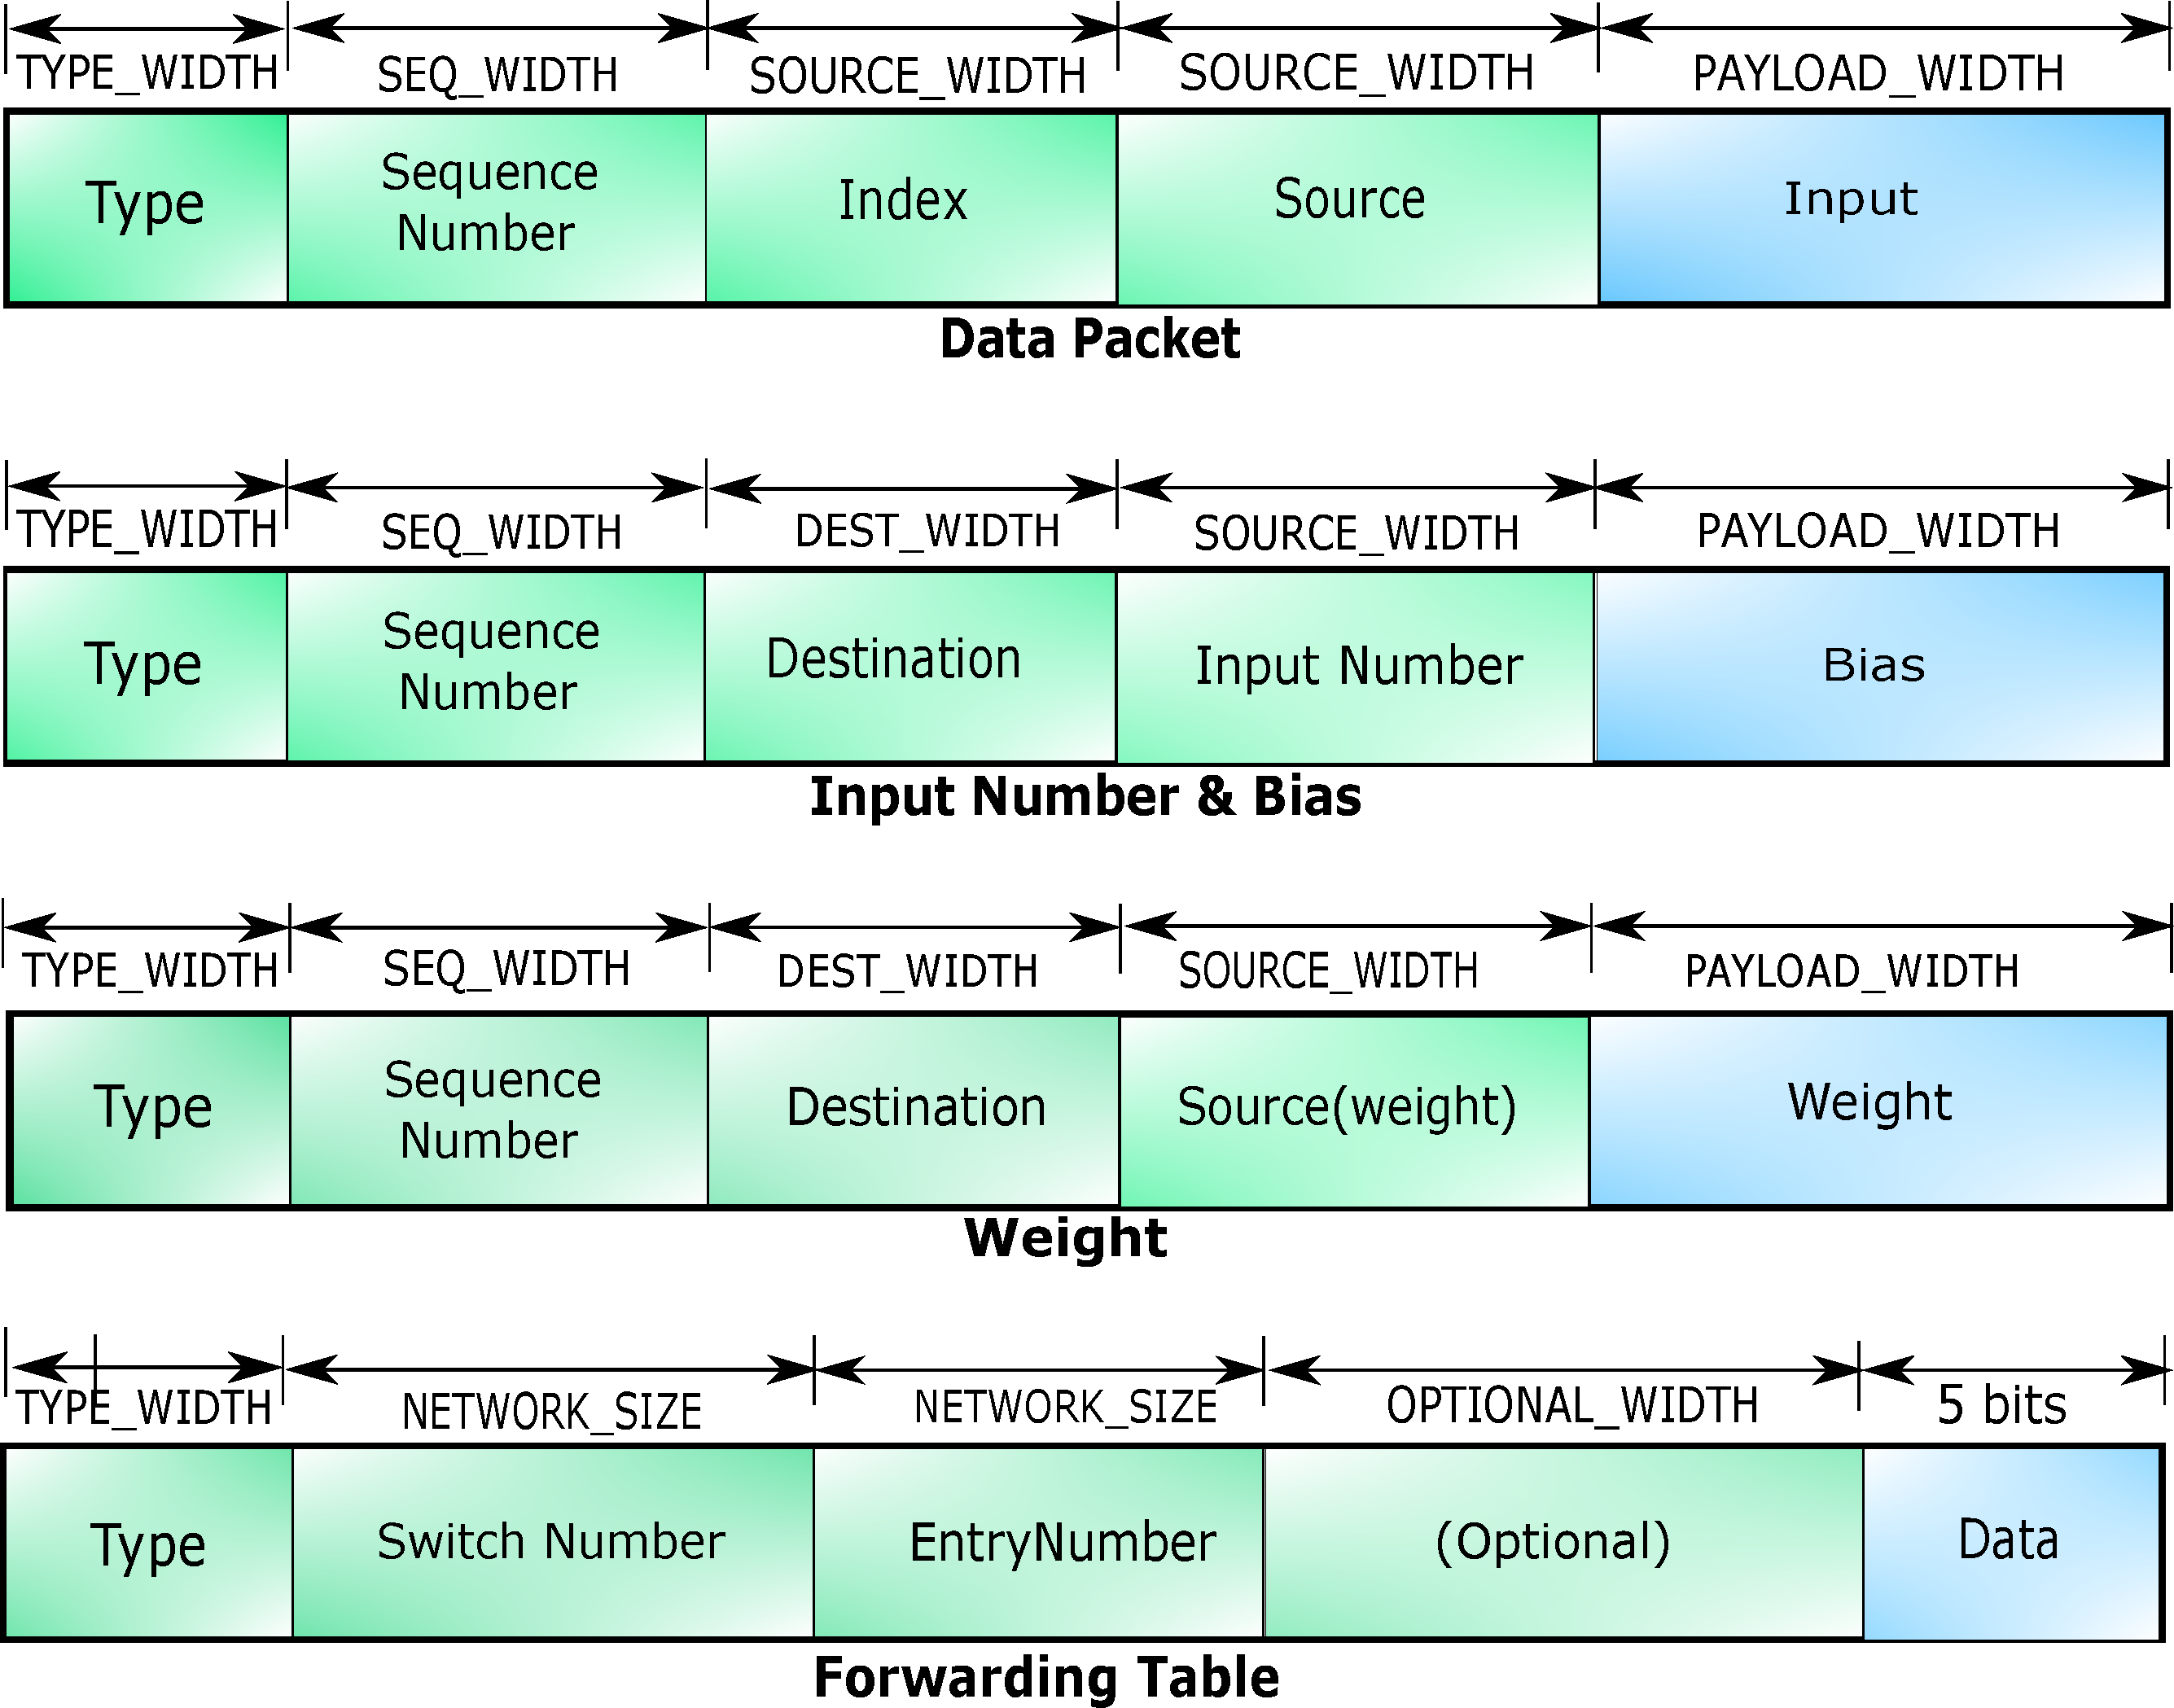
\includegraphics[width=0.8\columnwidth]{Figures/pktformat.pdf}
    \caption{NeuroNoC packet formats for supporting neuron and network configurations and data communication} 
    \label{figure:pktformat}
\end{figure}

\subsubsection*{\bf Data Packet}
Data packets are used for inter-neuron communication.
Once a neuron receives data packets from all its predecessors, it calculates the output based on inputs, weight values, bias and the activation function.
It sends out another data packet with the output in the \emph{input} field and the neuron address in the \emph{source} field.
The index field has significance only when the packet source is zero (bottom-left) PE.
Since the entire input layer is modelled by this single PE, the index number differentiates the different neurons of this layer.
\subsubsection*{\bf Input number and Bias Configuration Packet}
This configuration packet is used for configuring two parameters of each neuron.
The \emph{Input Number} field configures the number of predecessors of the neuron from the previous layer.
The \emph{Bias} field sets the neuron bias for calculating its output.
The \emph{Destination} field is used by the NoC to route the packet to appropriate neurons. 
\subsubsection*{\bf Weight Configuration Packet}
The Weight Configuration Packet sets the weight value for each neuron by storing the \emph{Weight} field in its internal Weight Table.
The \emph{Source} field enables mapping a a particular weight with a particular input.
Infact the Source field is used as the write address when storing weight in the weight table.
\subsubsection*{\bf Routing Table Configuration Packet}
These packets are used for configuring the NoC switch routing tables, enabling multicast routing algorithm described in subsection~\ref{}.

\subsection{Artificial Neuron}
Individual neurons of the NN are implementing by the processing elements (PEs) of the NoC.
Each neuron receives input from neurons in the previous layer, multiplies each input with corresponding weight, sums up and generates the output based on an activation function.
During configuration stage, each neuron is configured with the number of input neurons, weights corresponding each input and bias.
Fig.~\ref{fig:neuron} shows the different submodules of an artificial neuron and are described in the subsequest sections.
\subsubsection{\bf Sequence Number (SNC)}
 
Since packet switched NoC does not preserve packet ordering, neurons support out-of-order packet delivery by storing and reassembling the incoming data packets. 
The input layer (bottom-left PE) assigns each data packet a sequence number in the \emph{sequence number} field. 
It is to be noted that the number assigned corresponds to an input number rather than to a single packet.
In other words an input with \emph{n-feature vector space} will be sent as n packets with same sequence number. 
After processing the input data, the output packet from neurons retains sequence number of the input packets. 

\begin{figure}
    \centering
    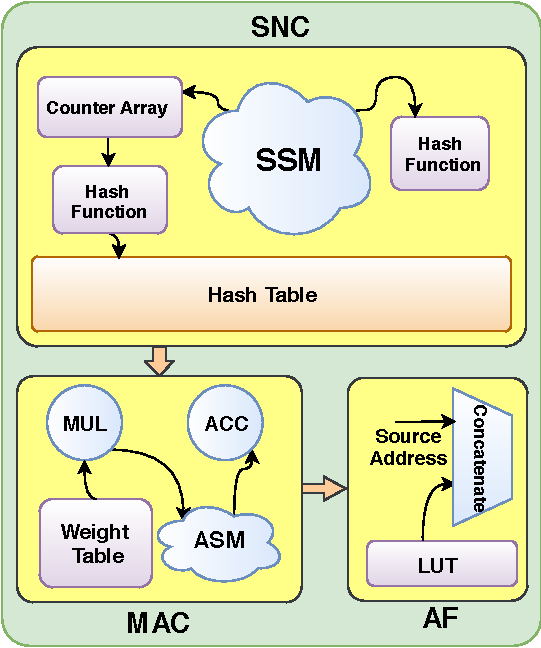
\includegraphics[width =0.8\columnwidth]{Figures/overall2.pdf}
    \caption{Architecture of the proposed artificial neuron}
    \label{fig:neuron}
\end{figure}

The data packets arriving from the network interface are initially stored in a hash table~(HT). 
The table consists of $2^{SEQ\_WIDTH}$ blocks, where $SEQ\_WIDTH$ amounts to the number of bits in the seqNum field. 
For a given NoC of size $S_{NOC}$, in the worst case each neuron may receive inputs from $S_{NOC}$ neighboring neurons. 
Thus, every block in HT is further divided to $S_{NOC}$ memory units. 
The data packets are mapped to HT memory through the following hash function,

\begin{equation}
hf(seqNum,count[seqNum]) = concat(seqNum,count[seqNum])
\label{equation:hf}
\end{equation}

Where \emph{count[seqNum]} is the number of packets with the same sequence number already received by the neuron.
The sequence number count is traked by the counter array (CR), which has a dedicated counter for each sequence number. 
After a packet is stored in the HT, the corresponding sequence number counter is incremented, so that the next packets with the same sequence number is stored in the next memory location. 
The SNC State Machine (SSM) tracks current sequence number and counter to retrieve packets from the HT. 

\subsection{Multipy-Accumulate Unit (MAC)}
The computation of the total synaptic input to the neuron constitutes the principal arithmetic operation to be implemented in a hardware design of a neural network. 
This is done by successive multiplication and addition operators i.e. a series of Multiply-Accumulate (MAC) operations. 
The reassembled packets from SNC are ushered towards Multiplication (MUL) stage. 
The weights are associated with the individual input packets through their source address, and these weights are stored in a Weight Table (WT) memory block which is shown in figure~\ref {figure:mac}. 
The weights can be configured on the run by sending corresponding control packets. 
The resultant product is accumulated at the Accumulation (ACC) stage. 
Assuming same format for neuron input and output data, the number of bits to represent weighted sum is

\begin{equation}
N_{s}=\lceil\log_{2}(S_{NOC}\cdot (2^{n_{w}-1})(2^{n_{z}-1})+2^{n_{b}-1}\cdot 2^{f_{z}+f_{w}+f_{b}})\rceil+1
\label{equation:Ns}
\end{equation}

The number of inputs and bias are configured with the same control packets which were used during SNC.  

\subsection{Activation Function (AF)}
The ANN implementation supports variety of activation functions with the help of look-up-tables~(LUTs).
By changing the contents of the LUT, the activation function can be modified.
LUT-based implementation of a complex and non-linear activation function, such as sigmoid function, may require large memory depending on the desirable precision.  
If we define $n_{s}$ as the most significant bits of $N_{s}$, increasing the value of $n_{s}$ contributes to the accuracy of the LUT at the expense of memory size. 
The minimum value at which all the possible output values are present in the LUT is given by

\begin{equation}
n_{s}=i_{s}-\lceil\log_{2}(\frac{d_{z}(1)}{{f}'(0)})\rceil
\label{equation:ns}
\end{equation}

Furthermore, if we consider sigmoid function, most of the entries located too far away from 0 are replicated. 
With this in mind, it is possible to reduce the size of LUT to store the central interval $[x_{high}, x_{low}]$, in where expressions for $x_{min}$ $x_{max}$ are given by

\begin{equation}
x_{high}=d_{s}(\ln{2^{f_{z}-1}}), x_{low}=-x_{high}
\label{equation:interval}
\end{equation}

and the number of bits to address the LUT is 
$n_{LUT}=\lceil\log_{2}{(x_{high}-x_{low}+1)}\rceil$.
If the computed weighted sum falls within the central interval, then the output is taken from the LUT otherwise the output is assigned either 1 or 0. 

\subsection{Switch}
The inner architecture of one switch is depicted in figure ~\ref{figure:switch_architecture}. Each switch able to send and accept packets from five direction: North, South, East, West and PE. In other words, switch can communicate with upper, lower, right, left neighboring switches and with own PE. Each direction has two FIFO for receiving and transmitting the data. The FIFO was implemented by using IP FIFO generator, therefore, the depth of them can be customized. Switches serve the FIFOs in a queue in a clockwise direction.  Flow control is implemented through AXI-stream control signal as shown if figure.  The $o\_valid$ wires are asserted whenever switch transmits the data for certain direction including PE. Similarly, whenever the data comes from other switches or PE the $i\_valid$ wire of incoming side of the switch is asserted. The switch asserts the $o\_ready$ signal whenever the FIFO has empty slot to accept the data. All FIFOs should hold the data on the bus until data is transmitted to all necessary FIFO. Each switch has registers for routing table, size of total size of NoC rows with 5 bits length. Switch has finite state machine controller, which routes the packet for certain directions depending on the packet type and refreshes the routing table. In one process time one packet can be transmitted to several FIFOs. Switches communicate with each other through FIFOs.  

\begin{figure}
    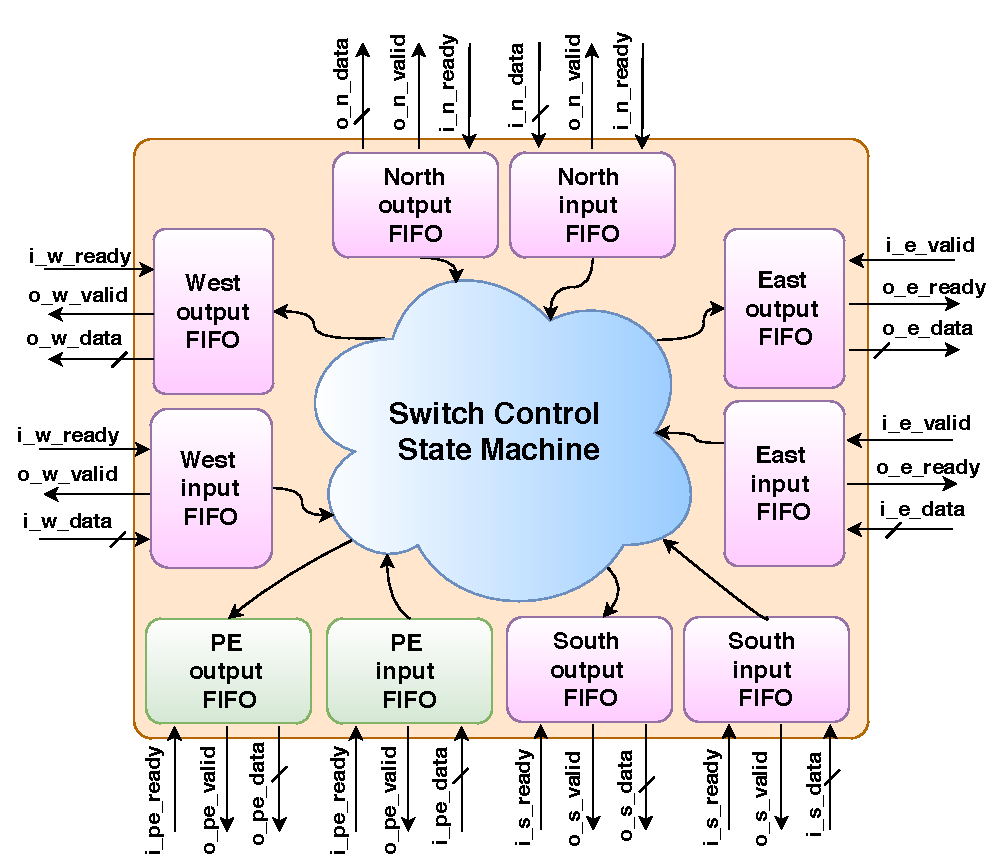
\includegraphics[width=\columnwidth]{Figures/switch2.pdf}
    \caption{Switch Architecture} 
    \label{figure:switch_architecture}
\end{figure}

\subsection{Routing Packets}
 Switch receives the packet from one FIFO and routes the data for required FIFOs. Finite state machine controller has three main approaches for routing the packets depending on the type of incoming packet.
 For weight and bias configuration packet switch sends the packet using the number of switch in the NoC. Depending on the number of destination switch, the present switch can route the packet for four directions. If the destination switch is located to the above, below, to the left or the right, it sends to North,South, East, West FIFOs respectively. Once the packet came to the predefined switch, instantly it will be sent to the PE FIFO corresponding to that switch for configuring the weight and bias.   
For routing table configuration packets switches behave the same as for weight and bias configuration oriented switches. The one difference is, when the packet came to the destination switch, it will refresh one slot of routing table and switch will serve next FIFO. 

While previous packets can be sent only for one direction(unicast) from one switch, the data packets can be replicated and sent for all direction including PE in one process time (multicast). It was achieved by the logic of routing table. Each switch has routing table, which must be configured before usage. The rows in routing table is equal to the total amount of switches in NoC. The actual meaning of rows in routing table is address of source switch. Whenever data packet comes, switch checks the source provider address of this packet and takes the row, which number is equal to source address. Each row has 5 bits for the decision to sending the packet for certain direction.  Each bit corresponds to 5 directions: North, South, East, West and PE. If the bit is equal to 1 then the incoming packet must be sent to corresponding direction,conversely, if bit is equal to 0 then the packet must not be sent to that direction. The routing table configuration directly depends on the neural network model and configuration packets must be created manually or using other software. For reliability of data in multicasted transmission, switch waits until the data is sent for all necessary direction, only after that it checks next FIFO. For implementation of packet routing the finite state machine principle was used and it is shown in figure ~\ref{figure:fsm}.


